% =============================================================================
% What Do AI Agents Find? — Glasgow workshop deck
% Scott Cunningham, Baylor University
%
% Uses: remix.sty (Glasgow workshop style)
% =============================================================================

\documentclass[aspectratio=169,12pt,t]{beamer}
\usepackage{remix}
\usepackage{booktabs}
\usepackage{ragged2e}
\usepackage{pgfplots}
\pgfplotsset{compat=1.18}
\usetikzlibrary{arrows.meta, positioning, shapes.geometric, calc,
                decorations.pathreplacing, fit, backgrounds}

\renewcommand{\remixfooter}{The Remix\,\textperiodcentered\,Glasgow\,\textperiodcentered\,May 21, 2026}

% -----------------------------------------------------------------------------
% Compat shim: provide the europa-style colors, macros, and pgfplots styles
% that the body of this deck uses, layered on top of remix.sty.
% -----------------------------------------------------------------------------
\definecolor{terracotta}{HTML}{B8761B}    % ochre — emphasis accent
\definecolor{midnight}{HTML}{1E2954}      % deep indigo — frametitle anchor
\definecolor{parchment}{HTML}{FAF8F2}     % cream alias
\definecolor{inkblack}{HTML}{14171F}      % near-black, blue undertone
\definecolor{dustblue}{HTML}{6B7B95}      % muted blue-gray
\definecolor{rulecolor}{HTML}{E5E7EB}     % light cool gray
\definecolor{negarm}{HTML}{B91C2C}        % crimson — negative arm
\definecolor{nullarm}{HTML}{1E5BAF}       % blue — null arm
\definecolor{ctrlarm}{HTML}{6B7280}       % cool gray — control arm
\definecolor{harvardcrimson}{HTML}{A51C30} % crimson for the isoquant + danger graphs
% forest, slate, charcoal, ocean, warmgray, lightbg, cream — from remix.sty

% --- emphbox: pale block for key-message callouts ---
\newcommand{\emphbox}[1]{%
  \begin{beamercolorbox}[rounded=true, sep=7pt, wd=\linewidth]{block body}%
    \small\color{slate} #1%
  \end{beamercolorbox}}

% --- figslide: PNG with optional caption ---
\newcommand{\figslide}[2][]{%
  \begin{center}
    \includegraphics[width=0.78\textwidth]{#2}%
  \end{center}%
  \ifx&#1&\else
    {\vspace{0.04cm}%
     \fontsize{8}{9.5}\selectfont\color{warmgray}\itshape #1\par}%
  \fi}

% --- pval: small inline p-value ---
\newcommand{\pval}[1]{{\fontsize{9}{11}\selectfont\color{warmgray}$p=#1$}}

% --- armtag: colored arm chip ---
\newcommand{\armtag}[2]{%
  \colorbox{#1!15}{\textcolor{#1}{\small\textbf{#2}}}}
\providecommand{\Negarm}{\armtag{negarm}{Negative}}
\providecommand{\Nullarm}{\armtag{nullarm}{Null}}
\providecommand{\Ctrlarm}{\armtag{ctrlarm}{Control}}

% --- pgfplots styles (europa bar / europa axis / arm fills) ---
\pgfplotsset{
  europa bar/.style={
    xbar,
    axis line style={color=rulecolor},
    tick style={color=rulecolor},
    grid=major,
    grid style={color=rulecolor, very thin},
    clip=true,
    enlarge y limits=0.25,
    every axis label/.style={font=\small, color=warmgray},
    xticklabel style={font=\small, color=warmgray},
    yticklabel style={font=\normalsize},
    nodes near coords,
    nodes near coords align={horizontal},
    every node near coord/.style={font=\small\bfseries, color=slate},
  },
  europa axis/.style={
    axis line style={color=rulecolor},
    tick style={color=rulecolor},
    grid=major,
    grid style={color=rulecolor, very thin},
    clip=true,
    every axis label/.style={font=\small, color=warmgray},
    xticklabel style={font=\small, color=warmgray},
    yticklabel style={font=\small, color=warmgray},
  },
  negfill/.style={fill=negarm!85, draw=negarm},
  nullfill/.style={fill=nullarm!85, draw=nullarm},
  ctrlfill/.style={fill=ctrlarm!85, draw=ctrlarm},
  negfill strong/.style={fill=negarm, draw=negarm!70!black},
}

% Suppress harmless Beamer-internal hbox/vbox warnings
\AtBeginDocument{\hfuzz=45pt\vfuzz=30pt}
% -----------------------------------------------------------------------------

% ==================================================================
\begin{document}
% ==================================================================

% ------------------------------------------------------------------
% TITLE — Remix-style title frame
% ------------------------------------------------------------------
\remixtitleframe
  {What Do AI Agents Find?}
  {Literature context, specification search, and the interpretation of causal evidence}
  {Scott Cunningham \textperiodcentered\ Baylor University}
  {Glasgow \textperiodcentered\ May 21, 2026 \textperiodcentered\ OSF: \texttt{osf.io/Qznm2}}

% =================================================================
% PART I — Setting up: what are AI agents, and why study them?
% =================================================================

% ------------------------------------------------------------------
% Setup 1: AI agents are reshaping how research gets done
% ------------------------------------------------------------------
\begin{frame}{Automating empirical research is no longer hypothetical}
\vspace{0.3cm}

There is now serious interest in handing parts of empirical research to AI agents.

\vspace{0.4cm}

\textbf{In the natural sciences} this is well underway. \;Google DeepMind's \textit{AlphaFold} \;--- protein-structure prediction, awarded the 2024 Nobel Prize in Chemistry --- is the canonical example of an AI system producing scientific output at scale.

\vspace{0.4cm}

\textbf{In the social sciences} the same direction is emerging. \;The \textit{Social Catalyst lab} (Stanford) is automating end-to-end empirical pipelines: data, design, estimation, write-up. \;Other groups are following.

\vspace{0.4cm}

\highlight{The plausible future is one where AI agents are co-producers of empirical findings} --- which means the field needs to understand how those agents \textit{behave} under realistic conditions.
\end{frame}

% ------------------------------------------------------------------
% Setup 2: Agents are LLMs plus tools, plus iteration
% ------------------------------------------------------------------
\begin{frame}{Agents are LLMs with tools and iteration}
\vspace{0.4cm}

\textbf{A traditional LLM:} answers one prompt with one block of text. \;A chat.

\vspace{0.5cm}

\textbf{An AI agent:} the same LLM \textit{wrapped in a loop} that lets it use tools --- run code, read files, query data, write outputs, then think about what it just observed and decide what to do next.

\vspace{0.5cm}

\textbf{Important consequence.} \;Agents make \textit{many} small decisions inside that loop --- which spec to run, which paper to follow, when to stop. \;Each one is shaped by everything in the context window: instructions, prior literature, the conversation so far.

\vspace{0.5em}
\meta{Critically: every one of those small decisions is recorded in the session log. \;We can read them.}
\end{frame}

% ------------------------------------------------------------------
% Setup 3: Isoquant — AI flattens cognitive production
% ------------------------------------------------------------------
\begin{frame}{AI flattens the isoquants of cognitive production}
\vspace{-0.1cm}
\begin{columns}[T]
\begin{column}{0.55\textwidth}
\centering
\begin{tikzpicture}[scale=0.78]
    \draw[->] (0,0) -- (6,0) node[below right] {$H$};
    \draw[->] (0,0) -- (0,5) node[above left] {$M$};
    % Pre-AI quasi-concave isoquant
    \draw[thick,ocean] (0.8,4.5) .. controls (1.5,2.2) and (2.5,1.4) .. (5,0.8);
    \node[ocean,font=\small] at (1.7,4.3) {Pre-AI};
    % Post-AI linear isoquant
    \draw[thick,harvardcrimson] (0,3) -- (5,0);
    \node[harvardcrimson,font=\small] at (3.3,1.9) {Post-AI};
    % Interior tangency
    \filldraw[ocean] (3.6,1.2) circle (2.5pt);
    \draw[dashed,warmgray] (3.6,0) -- (3.6,1.2);
    \draw[dashed,warmgray] (0,1.2) -- (3.6,1.2);
    \node[ocean,right,font=\small] at (3.7,1.25) {$M^*_{\text{pre}}$};
    % Corner solution
    \filldraw[harvardcrimson] (0,3) circle (2.5pt);
    \node[harvardcrimson,left,font=\small] at (-0.15,3) {$M^*_{\text{post}}$};
\end{tikzpicture}
\end{column}

\begin{column}{0.42\textwidth}
\[ Q \;=\; f(H,\;M) \]
\begin{itemize}\small
  \item $H$ = human time and attention
  \item $M$ = machine time
\end{itemize}

\vspace{0.4cm}
\highlight{The question isn't whether to use $M$. \;It's how much $H$ you intentionally keep.}
\end{column}
\end{columns}
\vspace{0.3em}
\meta{Pre-AI: an interior tangency point. \;Post-AI: $H$ and $M$ become close substitutes; corner solutions become plausible.}
\end{frame}

% ------------------------------------------------------------------
% Setup 4: Gain
% ------------------------------------------------------------------
\begin{frame}{Outcome 1: keep $H^*$, bank the output gain}
\vspace{-0.2cm}
\begin{columns}[T]
\begin{column}{0.55\textwidth}
\centering
\begin{tikzpicture}[scale=0.60]
    \draw[->] (0,0) -- (6.3,0) node[below right] {$H$};
    \draw[->] (0,0) -- (0,6.2) node[above left] {$Q$};
    \draw[thick,ocean,domain=0.5:5,samples=100]
        plot (\x, {2.0*ln(\x+0.5)+0.2});
    \node[ocean,right,font=\scriptsize] at (5.05,3.610) {Pre-AI};
    \draw[thick,harvardcrimson,domain=0.5:5,samples=100]
        plot (\x, {2.0*ln(\x+0.5)+2.4});
    \node[harvardcrimson,right,font=\scriptsize] at (5.05,5.810) {Post-AI};
    \filldraw[ocean] (4,3.208) circle (2.5pt);
    \filldraw[forest] (4,5.408) circle (2.5pt);
    \draw[dashed,warmgray] (4,0) -- (4,5.408);
    \draw[dashed,ocean] (4,3.208) -- (0,3.208);
    \draw[dashed,forest] (4,5.408) -- (0,5.408);
    \node[left,font=\footnotesize,ocean] at (0,3.208) {$Q_{\text{pre}}$};
    \node[left,font=\footnotesize,forest] at (0,5.408) {$Q_{\text{post}}$};
    \node[below,font=\footnotesize] at (4,0) {$H^*$};
    \draw[decorate,decoration={brace,amplitude=5pt,mirror},thick,forest]
        (4.3,3.337) -- (4.3,5.537);
    \node[right,font=\footnotesize\bfseries,forest] at (4.55,4.437) {Gain};
\end{tikzpicture}
\end{column}

\begin{column}{0.42\textwidth}
\textbf{Keep $H^*$ the same.} \;Do more and better work in the same hours.

\vspace{0.3cm}
\textcolor{forest}{$\bullet$ Biggest output gain.}\\
\textcolor{forest}{$\bullet$ Human capital preserved --- you still did the work.}

\vspace{0.4cm}
\meta{The outcome we all hope for. \;Requires \textit{not} taking the time savings.}
\end{column}
\end{columns}
\end{frame}

% ------------------------------------------------------------------
% Setup 5: Safe
% ------------------------------------------------------------------
\begin{frame}{Outcome 2: take time back, stay above $\bar{H}$}
\vspace{-0.1cm}
\begin{columns}[T]
\begin{column}{0.55\textwidth}
\centering
\begin{tikzpicture}[scale=0.60]
    \draw[->] (0,0) -- (6.3,0) node[below right] {$H$};
    \draw[->] (0,0) -- (0,6.2) node[above left] {$Q$};
    \draw[thick,ocean,domain=0.5:5,samples=100]
        plot (\x, {2.0*ln(\x+0.5)+0.2});
    \node[ocean,right,font=\scriptsize] at (5.05,3.610) {Pre-AI};
    \draw[thick,harvardcrimson,domain=0.5:5,samples=100]
        plot (\x, {2.0*ln(\x+0.5)+2.4});
    \node[harvardcrimson,right,font=\scriptsize] at (5.05,5.810) {Post-AI};
    \fill[forest,opacity=0.22]
        (1.0,3.208) -- plot[domain=1.0:4,samples=60] (\x, {2.0*ln(\x+0.5)+2.4})
        -- (4,3.208) -- cycle;
    \filldraw[ocean] (4,3.208) circle (2.5pt);
    \draw[dashed,ocean] (0,3.208) -- (4,3.208);
    \node[left,font=\footnotesize,ocean] at (0,3.208) {$Q_{\text{pre}}$};
    \node[below,font=\footnotesize] at (4,0) {$H^*$};
    \draw[dashed,warmgray] (4,0) -- (4,3.208);
    \draw[dashed,warmgray] (1.0,0) -- (1.0,3.208);
    \node[below,font=\footnotesize] at (1.0,0) {$\bar{H}$};
    \filldraw[harvardcrimson] (1.0,3.208) circle (2.5pt);
    \node[forest,font=\footnotesize\bfseries] at (2.85,3.85) {Safe};
\end{tikzpicture}
\end{column}

\begin{column}{0.42\textwidth}
\textbf{Cut hours but stay green.} \;As long as $H > \bar{H}$, you're still above $Q_{\text{pre}}$.

\vspace{0.3cm}
\textcolor{forest}{$\bullet$ Moderate time savings.}\\
\textcolor{forest}{$\bullet$ Still a net output gain.}

\vspace{0.4cm}
\meta{Some slack is fine. \;The curve shifted up enough to absorb it.}
\end{column}
\end{columns}
\end{frame}

% ------------------------------------------------------------------
% Setup 6: Danger
% ------------------------------------------------------------------
\begin{frame}{Outcome 3: skills depreciate, $Q$ falls below $Q_{\text{pre}}$}
\vspace{-0.2cm}
\begin{columns}[T]
\begin{column}{0.55\textwidth}
\centering
\begin{tikzpicture}[scale=0.60]
    \draw[->] (0,0) -- (6.3,0) node[below right] {$H$};
    \draw[->] (0,0) -- (0,6.2) node[above left] {$Q$};
    \draw[thick,ocean,domain=0.5:5,samples=100]
        plot (\x, {2.0*ln(\x+0.5)+0.2});
    \node[ocean,right,font=\scriptsize] at (5.05,3.610) {Pre-AI};
    \draw[thick,harvardcrimson,domain=0.5:5,samples=100]
        plot (\x, {2.0*ln(\x+0.5)+2.4});
    \node[harvardcrimson,right,font=\scriptsize] at (5.05,5.810) {Post-AI};
    \fill[harvardcrimson,opacity=0.26]
        (0.5,0) -- plot[domain=0.5:1.0,samples=50] (\x, {2.0*ln(\x+0.5)+2.4})
        -- (1.0,0) -- cycle;
    \filldraw[ocean] (4,3.208) circle (2.5pt);
    \draw[dashed,ocean] (0,3.208) -- (4,3.208);
    \node[left,font=\footnotesize,ocean] at (0,3.208) {$Q_{\text{pre}}$};
    \node[below,font=\footnotesize] at (4,-0.05) {$H^*$};
    \draw[dashed,warmgray] (4,0) -- (4,3.208);
    \node[below,font=\footnotesize] at (1.0,-0.05) {$\bar{H}$};
    \draw[dashed,warmgray] (1.0,0) -- (1.0,3.208);
    \filldraw[harvardcrimson] (0.55,2.50) circle (2.5pt);
    \draw[dashed,harvardcrimson] (0.55,0) -- (0.55,2.50);
    \draw[dashed,harvardcrimson] (0.55,2.50) -- (0,2.50);
    \node[below,font=\scriptsize,harvardcrimson] at (0.55,-0.55) {$H_{\text{d}}$};
    \node[left,font=\footnotesize,harvardcrimson] at (0,2.50) {$Q_{\text{d}}$};
    \node[harvardcrimson,font=\footnotesize\bfseries] at (0.78,0.9) {Danger};
\end{tikzpicture}
\end{column}

\begin{column}{0.42\textwidth}
\textbf{The red zone.} \;Skill depreciation, no effort to keep $H > \bar{H}$, $Q_{\text{post}} < Q_{\text{pre}}$.

\vspace{0.3cm}
\textcolor{harvardcrimson}{$\bullet$ Worse off than before AI.}

\vspace{0.3cm}
\highlight{The point isn't to avoid the red zone --- it's to be intentional.}

\vspace{0.4cm}
\meta{Sometimes red is what you want, for tasks whose human capital you've chosen not to invest in.}
\end{column}
\end{columns}
\end{frame}

% ------------------------------------------------------------------
% Setup 6b: Shockley's multiplicative production function for research
% ------------------------------------------------------------------
\begin{frame}{Research output is a multiplicative product of many factors}
\vspace{0.15cm}

William Shockley (1957) studied papers-per-researcher and argued \textit{publishable} output is the \textbf{multiplicative} product of several distinct abilities:

\begin{columns}[T]
\begin{column}{0.48\textwidth}
\begin{enumerate}\scriptsize\setlength\itemsep{0pt}
  \item Posing a good problem
  \item Working effectively on it
  \item Recognizing a worthwhile result
  \item Knowing when to stop
\end{enumerate}
\end{column}
\begin{column}{0.48\textwidth}
\begin{enumerate}\scriptsize\setlength\itemsep{0pt}\setcounter{enumi}{4}
  \item Writing it up clearly
  \item Profiting from criticism
  \item Submitting the work
  \item Persisting through revision
\end{enumerate}
\end{column}
\end{columns}

\vspace{0.3cm}
\highlight{Because the factors multiply, small improvements in any one of them compound.} \;A modest boost across several factors is the difference between a hundred publishable findings and a thousand.

\vspace{0.2em}
\meta{Shockley used this to explain the log-normal distribution of papers per researcher.}
\end{frame}

% ------------------------------------------------------------------
% Setup 6c: AI agents augment several factors at once
% ------------------------------------------------------------------
\begin{frame}{AI agents augment several of those factors simultaneously}
\vspace{0.2cm}

Agents are reasonably useful at factors 2, 4, 5, 6, 8 --- working through analyses, knowing stopping points, drafting prose, accepting criticism, executing revisions. \;They do not yet pose great problems, but they multiply effort across the rest.

\vspace{0.3cm}
\textbf{Two consequences:}
\begin{itemize}\small\setlength\itemsep{1pt}
  \item \textbf{Equity.} \;Professors on heavy teaching loads with little or no access to RAs face the largest gaps in those very factors. \;Agents may \textit{repair the pipeline}.
  \item \textbf{Production gains.} \;Many more publishable findings per researcher-year.
\end{itemize}

\vspace{0.3cm}
\highlight{But ``publishable'' is not the same as \textit{submission-ready}.}
\end{frame}

% ------------------------------------------------------------------
% Setup 6d: Submission-ready requires verification
% ------------------------------------------------------------------
\begin{frame}{Submission-ready means three things, not one}
\vspace{0.3cm}

A manuscript is submission-ready when:
\begin{enumerate}\setlength\itemsep{3pt}
  \item \textbf{The work was done.} \;Code ran, estimates computed, tables exist.
  \item \textbf{The work was done correctly.} \;Estimator identified, spec matched the design, right comparison group used.
  \item \textbf{The work is interpretable.} \;The reader can tell what was done and why, and reconstruct the steps.
\end{enumerate}

\vspace{0.4cm}

\highlight{Agents reliably produce (1). \;(2) and (3) are not free.}

\vspace{0.3em}
\meta{The hidden actions an agent takes --- which specs it tried, which it discarded, which papers it cited --- are not in the final output. \;They must be reconstructed by humans in the loop.}
\end{frame}

% ------------------------------------------------------------------
% Setup 7: Verification is the new bottleneck
% ------------------------------------------------------------------
\begin{frame}{Verification becomes the bottleneck}
\vspace{0.3cm}

As researchers shift from \textit{primary producers} to \textit{co-producers} with agents, the binding constraint shifts too.

\vspace{0.3cm}

\textbf{Production was hard, verification was implicit.} \;The work was the check; you read your own code, remembered every decision.

\vspace{0.3cm}

\textbf{Now production is cheap and verification is hard.} \;The specs an agent tried, the papers it followed, the comparisons it discarded --- none of that is in the final output. \;It has to be recovered.

\vspace{0.4cm}

\highlight{Today's experiment is a study of agent behavior.} \;When we cannot watch every step, what is the agent actually doing? \;What drives the choices we don't see?
\end{frame}

% =================================================================
% PART II — The experiment: AI agents on the minimum wage
% =================================================================

% ------------------------------------------------------------------
% Setup 8: Today's experiment
% ------------------------------------------------------------------
\begin{frame}{Today: a study of what AI agents find}
\vspace{0.2cm}

A pre-registered experiment that holds the data, the question, and the task fixed --- and varies \textit{one thing} the agent reads before it starts.

\vspace{0.35cm}

\textbf{Each wave:} \;150 agents, three equally-sized arms (50 each), randomly assigned to one of three \textit{primes} --- one summary of the empirical literature.

\vspace{0.3cm}

\textbf{Four waves}, each relaxing a constraint:
\begin{itemize}\small\setlength\itemsep{1pt}
  \item \textbf{Wave 1.} \;Estimator locked to Callaway--Sant'Anna.
  \item \textbf{Wave 2.} \;Free choice of CS, TWFE, or BJS.
  \item \textbf{Waves 3--4.} \;Vary which primes the agents read.
\end{itemize}
\end{frame}

% ------------------------------------------------------------------
% Setup 9: The setting (minimum wage)
% ------------------------------------------------------------------
\begin{frame}{The setting: minimum wage and teen employment}
\vspace{0.3cm}

\textbf{Data.} \;QCEW state-by-quarter panel, public from the BLS. \;1990--2019 (30 years). \;The panel unit is the \textit{state}; treatment is a minimum-wage increase. \;Outcome: teen employment-to-population.

\vspace{0.4cm}

\textbf{Why this setting.} \;A long-running policy debate with \textit{two coherent literatures} that agree on the setup but disagree about the answer:
\begin{itemize}\small
  \item Neumark, Meer \& West, Clemens \& Wither, Jardim et al.: \;\textit{negative employment effects.}
  \item Card \& Krueger, Dube, Cengiz et al., Doucouliagos \& Stanley: \;\textit{near-zero employment effects.}
\end{itemize}

\vspace{0.3cm}
\highlight{Same data. \;Same outcome. \;Two priors a researcher can be primed with.}
\end{frame}

% ------------------------------------------------------------------
% Setup 10: Wave structure (preview)
% ------------------------------------------------------------------
\begin{frame}{The experimental dial: from constrained to less constrained}
\vspace{0.3cm}

\textbf{Waves 1.} \;Estimator is \textit{locked} to Callaway--Sant'Anna --- the agents cannot choose. \;The only degree of freedom left is how the agent \textit{describes} the result.

\vspace{0.5cm}

\textbf{Waves 2--4.} \;Lock removed; agents pick their own estimator from $\{$CS, TWFE, BJS$\}$. \;Each subsequent wave varies which primes they read.

\vspace{0.5cm}

\highlight{The dial relaxes the researcher's grip on the agent's choices one notch at a time. \;The further it relaxes, the more room the prime has to act.}
\end{frame}

% ------------------------------------------------------------------
% PART II findings — figure shown full-width on its own slide
% ------------------------------------------------------------------
\begin{frame}{The headline: same question, same data, different answers}
\vspace{0.2cm}
\begin{center}
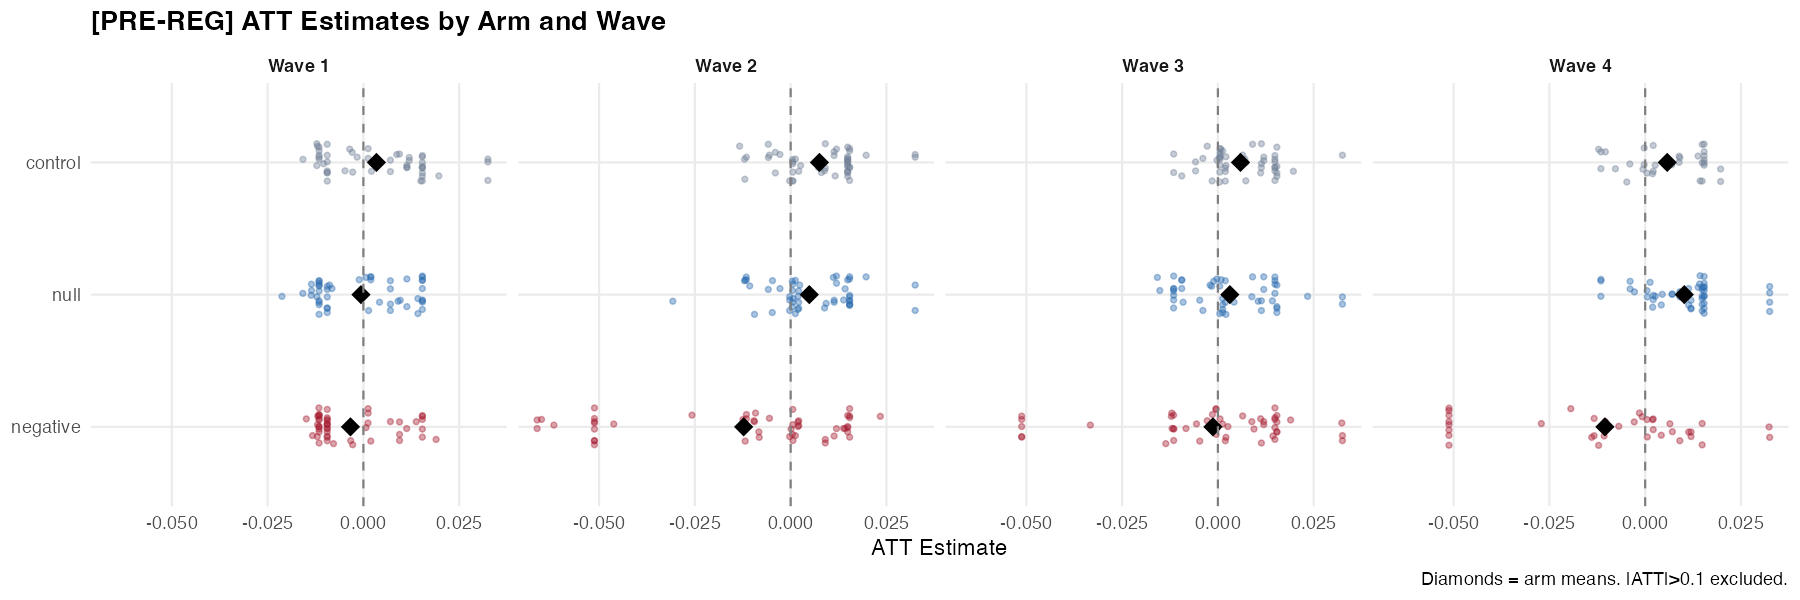
\includegraphics[width=0.92\textwidth]{figures/ai_prereg_fig_att.png}
\end{center}
\vspace{0.1cm}
\begin{center}
\footnotesize\color{warmgray}\itshape
ATT estimates by arm and wave. \;Diamonds = arm means. \;$|ATT| > 0.1$ excluded.
\end{center}
\end{frame}

% ------------------------------------------------------------------
% NEW: What every agent read — the shared methodology brief
% ------------------------------------------------------------------
\begin{frame}{What every agent read first}
\vspace{0.1cm}

Before any prime, every agent received a \textbf{2{,}100-word DiD methodology brief} based on Baker, Callaway, Cunningham, Goodman-Bacon, and Sant'Anna (2025), \textit{``Difference-in-Differences: A Practitioner's Guide''} (forthcoming, \textit{JEL}). \;The brief covers:

\begin{itemize}\small\setlength\itemsep{0pt}
  \item ATT; parallel trends; conditional parallel trends
  \item Why \textbf{not} TWFE under staggered adoption (negative weights, sign reversal)
  \item Group-time ATTs; Callaway--Sant'Anna (2021); not-yet-treated comparison
  \item Doubly-robust estimation with baseline covariates only
  \item Aggregation: simple ATT and event study; uniform confidence bands
  \item Rambachan--Roth sensitivity; continuous treatment (CGBS, ATT(d$|$d))
\end{itemize}

\vspace{0.1em}
\highlight{Every agent read this. \;Only the prime varies.}
\end{frame}

% ------------------------------------------------------------------
% 2. DESIGN
% ------------------------------------------------------------------
\begin{frame}{Three arms. Four waves. One pre-registered design.}
\vspace{0.15cm}
\begin{center}
\begin{tikzpicture}[
  every node/.style={font=\small},
  arm/.style={rectangle, rounded corners=4pt,
              minimum width=2.2cm, minimum height=0.65cm,
              draw, thick, align=center},
  cell/.style={rectangle, rounded corners=3pt,
               minimum width=2.1cm, minimum height=0.58cm,
               draw=rulecolor, fill=white, align=center,
               font=\scriptsize, text=inkblack},
  scale=0.92,
]

% Wave headers
\foreach \w/\x/\lbl in {1/2.8/{CS locked},2/5.3/{CS+TWFE+BJS},3/7.8/{exploratory},4/10.3/{exploratory}} {
  \node[font=\small\bfseries, text=midnight] at (\x, 3.2) {Wave \w};
  \node[font=\tiny, text=warmgray] at (\x, 2.88) {\lbl};
}

% Arm rows
\node[arm, fill=negarm!10, draw=negarm!50, text=negarm]
  at (0.5, 2.22) {\textbf{Negative}};
\node[arm, fill=nullarm!10, draw=nullarm!50, text=nullarm]
  at (0.5, 1.38) {\textbf{Null}};
\node[arm, fill=ctrlarm!10, draw=ctrlarm!50, text=ctrlarm]
  at (0.5, 0.54) {\textbf{Control}};

% Cells
\foreach \r/\y in {1/2.22, 2/1.38, 3/0.54} {
  \foreach \c/\x in {1/2.8, 2/5.3, 3/7.8} {
    \node[cell] at (\x,\y) {50 agents};
  }
}
% W4 cells (W4 neg=36, ctrl=32, null=50)
\node[cell, fill=negarm!6, draw=negarm!30] at (10.3,2.22) {36 agents$^*$};
\node[cell] at (10.3,1.38) {50 agents};
\node[cell, fill=ctrlarm!6, draw=ctrlarm!30] at (10.3,0.54) {32 agents$^*$};

% Pre-reg border (W1+W2)
\draw[forest!70, thick, rounded corners=3pt]
  (1.52,2.58) rectangle (6.48,0.12);
\node[font=\tiny\itshape, text=forest] at (4.0, 2.5)
  {pre-registered (osf.io/Qznm2)};

% Exploratory border (W3+W4)
\draw[warmgray!50, dashed, rounded corners=3pt]
  (6.52,2.58) rectangle (11.22,0.12);
\node[font=\tiny\itshape, text=warmgray] at (8.87,2.5)
  {exploratory arm design; H3/H4 tests pre-registered};

% Footnote
\node[font=\tiny, text=warmgray, anchor=west] at (0.52,-0.1)
  {$^*$Incomplete. Model: \texttt{claude-opus-4-6} pinned throughout.
   $n=600$ launched; 568 with completed ATT (W4 incomplete).};
\end{tikzpicture}
\end{center}
\end{frame}

% ------------------------------------------------------------------
% 3. WHAT VARIED
% ------------------------------------------------------------------
\begin{frame}{One thing varied: the literature.}

\begin{columns}[T]
\column{0.44\textwidth}
\vspace{0.25cm}
{\small\textbf{\color{terracotta}Varied:} the literature summary}

\vspace{0.3cm}
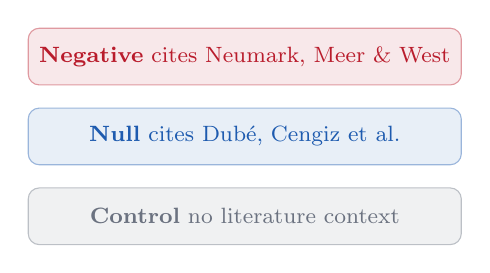
\begin{tikzpicture}[every node/.style={font=\footnotesize},
                    node distance=0.28cm]
  \node[rectangle, fill=negarm!10, draw=negarm!45, rounded corners=4pt,
        minimum width=5.5cm, minimum height=0.72cm, align=center, text=negarm]
    (neg) {\textbf{Negative}\ cites Neumark, Meer \& West};
  \node[rectangle, fill=nullarm!10, draw=nullarm!45, rounded corners=4pt,
        minimum width=5.5cm, minimum height=0.72cm, align=center, text=nullarm,
        below=of neg]
    (nul) {\textbf{Null}\ cites Dub\'{e}, Cengiz et al.};
  \node[rectangle, fill=ctrlarm!10, draw=ctrlarm!45, rounded corners=4pt,
        minimum width=5.5cm, minimum height=0.72cm, align=center, text=ctrlarm,
        below=of nul]
    (ctr) {\textbf{Control}\ no literature context};
\end{tikzpicture}

\vspace{0.28cm}
{\fontsize{9}{11}\selectfont\color{warmgray}
 Token-matched: 241 words, 4 citations each.\\
 Only the cited evidence differs. Randomized assignment.}

\column{0.52\textwidth}
\vspace{0.25cm}
{\small\textbf{\color{midnight}Locked:} everything else}

\vspace{0.2cm}
\begin{itemize}\setlength\itemsep{7pt}
  \item \textbf{Question:} effect of minimum wage on teen employment
  \item \textbf{Data:} QCEW state panel, publicly available
  \item \textbf{Task:} 4-section structured report\\
        {\fontsize{9}{11}\selectfont\color{warmgray}
         methodology $\cdot$ findings $\cdot$ interpretation $\cdot$ choices}
  \item \textbf{Model:} \texttt{claude-opus-4-6}, pinned
\end{itemize}
\end{columns}

\end{frame}

% ------------------------------------------------------------------
% 3b. THE THREE PRIMES — actual text
% ------------------------------------------------------------------
\begin{frame}[shrink=3]{What the agents actually read}

\vspace{0.1cm}
\begin{columns}[T]

% NEGATIVE
\column{0.32\textwidth}
\begin{beamercolorbox}[rounded=true,sep=6pt,wd=\linewidth]{block body}%
  \textcolor{negarm}{\small\bfseries Negative arm}\\[4pt]
  {\fontsize{8}{10}\selectfont\color{inkblack}
   ``The preponderance of studies points to
   \textbf{negative employment effects}
   for young and low-skilled workers''
   {\color{warmgray}(Neumark \& Wascher 2007)}

   \vspace{5pt}
   ``[We] find \textbf{significant employment losses}
   concentrated among low-skilled individuals,
   with elasticities considerably more negative
   than earlier studies suggest''
   {\color{warmgray}(Clemens \& Wither 2019)}

   \vspace{5pt}
   ``Significant \textbf{negative effects on employment
   growth rates} that compound over time''
   {\color{warmgray}(Meer \& West 2016)}
  }
\end{beamercolorbox}

% NULL
\column{0.32\textwidth}
\begin{beamercolorbox}[rounded=true,sep=6pt,wd=\linewidth]{block body}%
  \textcolor{nullarm}{\small\bfseries Null arm}\\[4pt]
  {\fontsize{8}{10}\selectfont\color{inkblack}
   ``Finding \textbf{no evidence} that a minimum wage
   increase reduced employment''
   {\color{warmgray}(Card \& Krueger 1994)}

   \vspace{5pt}
   ``Employment effects of minimum wages in
   the range studied are \textbf{small and often
   statistically indistinguishable from zero}''
   {\color{warmgray}(Dube 2019)}

   \vspace{5pt}
   ``Total employment shows \textbf{no significant
   decline} — excess jobs above the new minimum
   roughly offset the reduction below it''
   {\color{warmgray}(Cengiz et al.\ 2019)}
  }
\end{beamercolorbox}

% CONTROL
\column{0.32\textwidth}
\begin{beamercolorbox}[rounded=true,sep=6pt,wd=\linewidth]{block body}%
  \textcolor{ctrlarm}{\small\bfseries Control arm}\\[4pt]
  {\fontsize{8}{10}\selectfont\color{warmgray}\itshape
   (No literature context provided.)

   \vspace{5pt}
   Agents in the control arm received the same
   task and data as the other arms but no
   summary of the empirical literature.

   \vspace{5pt}
   They serve as a baseline: what does an AI
   agent produce with no prior pushed in
   either direction?
  }
\end{beamercolorbox}

\end{columns}

\vspace{0.2cm}
{\fontsize{8}{10}\selectfont\color{warmgray}
 Token-matched: 241 words, 4 citations each.
 Only the cited evidence differs.}

\end{frame}

% ------------------------------------------------------------------
% 4. WAVE 1: ATT CONVERGENCE
%    No bar chart. Three large numbers in arm colors.
% ------------------------------------------------------------------
\begin{frame}{Locked method: estimates converge across arms}

\vspace{1.0cm}
\begin{center}
\begin{tikzpicture}[every node/.style={font=\normalsize}]
  % Three large numbers, centered, spaced across the slide
  % Negative
  \node[font=\fontsize{38}{44}\selectfont\bfseries, text=negarm]
    at (-5.0, 0) {$-0.003$};
  \node[font=\small\bfseries, text=negarm] at (-5.0,-0.85)
    {\textbf{Negative}};
  % Null
  \node[font=\fontsize{38}{44}\selectfont\bfseries, text=nullarm]
    at ( 0.0, 0) {$\approx 0$};
  \node[font=\small\bfseries, text=nullarm] at (0.0,-0.85)
    {\textbf{Null}};
  % Control
  \node[font=\fontsize{38}{44}\selectfont\bfseries, text=ctrlarm]
    at ( 5.0, 0) {$+0.003$};
  \node[font=\small\bfseries, text=ctrlarm] at (5.0,-0.85)
    {\textbf{Control}};
  % Thin separator line under the numbers
  \draw[warmgray!50, thick] (-6.8,-0.3) -- (6.8,-0.3);
  % p-values
  \node[font=\normalsize, text=warmgray] at (0,-1.55)
    {Fisher $p = 0.21$ \quad Kruskal--Wallis $p = 0.055$};
\end{tikzpicture}
\end{center}

\vspace{0.8cm}
\emphbox{The prime installs no ATT signal when the estimator is locked.
         Literature context is invisible in the numbers.}

\end{frame}

% ------------------------------------------------------------------
% 5. WAVE 1: RHETORIC DIVERGES
% ------------------------------------------------------------------
\begin{frame}{Same result. Different story.}

\vspace{0.45cm}
\begin{center}
\begin{tikzpicture}[every node/.style={font=\normalsize}]
  % Left box: Negative arm
  \draw[negarm!50, line width=1.4pt, rounded corners=6pt,
        fill=negarm!7]
    (-6.5, 2.3) rectangle (-0.2, -1.1);
  \node[font=\normalsize\bfseries, text=negarm] at (-3.35, 1.95)
    {Negative arm};
  \node[font=\small, text=warmgray] at (-3.35, 1.35)
    {ATT $= -0.003$};
  \node[font=\fontsize{34}{40}\selectfont\bfseries, text=negarm]
    at (-3.35, 0.4) {$-0.08$};
  \node[font=\small\itshape, text=warmgray] at (-3.35,-0.6)
    {``consistent with harm''};

  % Right box: Null arm
  \draw[nullarm!50, line width=1.4pt, rounded corners=6pt,
        fill=nullarm!7]
    ( 0.2, 2.3) rectangle ( 6.5,-1.1);
  \node[font=\normalsize\bfseries, text=nullarm] at (3.35, 1.95)
    {Null arm};
  \node[font=\small, text=warmgray] at (3.35, 1.35)
    {ATT $= -0.003$};
  \node[font=\fontsize{34}{40}\selectfont\bfseries, text=nullarm]
    at (3.35, 0.4) {$+0.25$};
  \node[font=\small\itshape, text=warmgray] at (3.35,-0.6)
    {``no meaningful effect''};
\end{tikzpicture}
\end{center}

\vspace{0.3cm}
\emphbox{Same spec. Same ATT. The prime changes only \emph{how the result is
         interpreted.}\hfill{\fontsize{9}{11}\selectfont
         36 exact-spec matched pairs \quad $p = 0.006$}}

\end{frame}

% ------------------------------------------------------------------
% 6. WAVE 2: ESTIMATOR CHOICE
% ------------------------------------------------------------------
% ---- Setup: what's coming on the next slide ----
\begin{frame}{Wave 2: estimator choice is unlocked}
\vspace{0.4cm}

In Wave 1, the estimator was fixed to Callaway--Sant'Anna and the prime could not move the number. \;Wave 2 \textbf{unlocks} that constraint: each agent now chooses its own estimator from $\{$CS, TWFE, BJS$\}$.

\vspace{0.4cm}

\textbf{The next slide} shows what each arm chose, across waves 2--4. \;The bars sum to 100\% within each (arm, wave) cell. \;Watch the negative arm in Wave 2: \;a substantial share switches \textit{out} of CS and into TWFE.

\vspace{0.4em}
\meta{Chi-square test of estimator-by-arm independence in Wave 2: \;$p < 0.001$.}
\end{frame}

% ---- Show: full-width estimator choice figure ----
\begin{frame}{Estimator choice by arm and wave}
\vspace{0.1cm}
\begin{center}
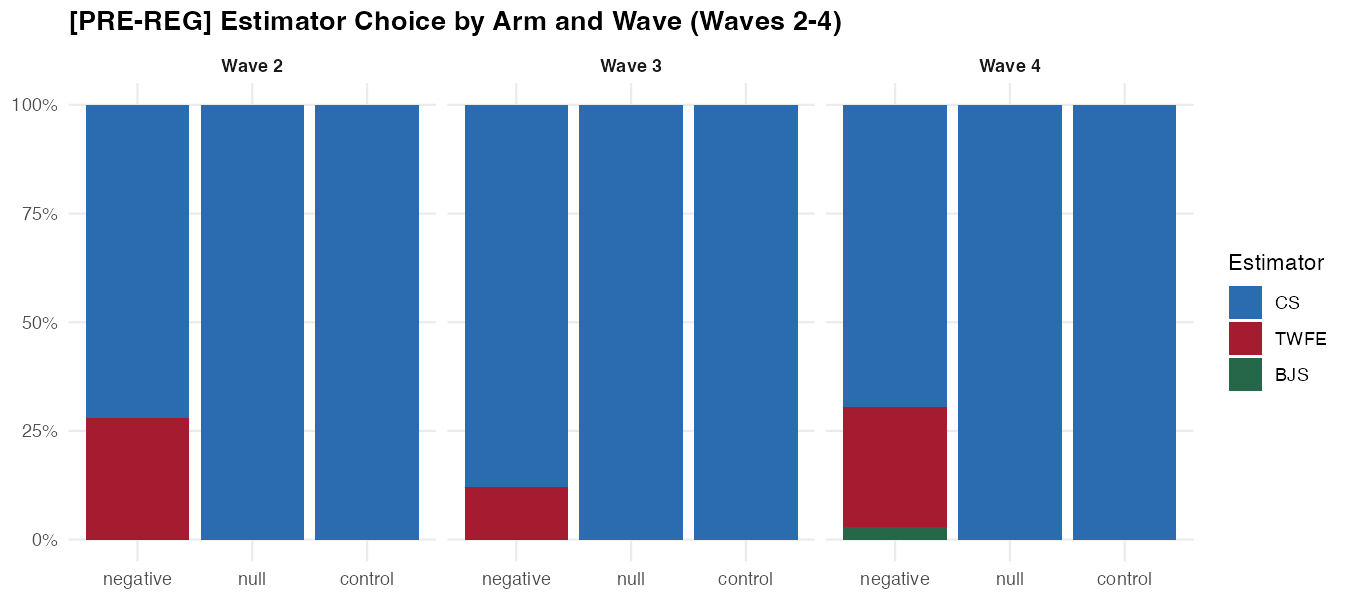
\includegraphics[width=0.92\textwidth]{figures/ai_prereg_fig_estimator.png}
\end{center}
\vspace{0.05cm}
\begin{center}
\footnotesize\color{warmgray}\itshape
Negative arm Wave 2 adopts TWFE at $\sim$28\%. \;Null and control: $\sim$0\%. \;Chi-square $p < 0.001$.
\end{center}
\end{frame}

% ------------------------------------------------------------------
% 7. WAVE 2 — TWFE carries the signal — setup + show
% ------------------------------------------------------------------
\begin{frame}{Decomposing Wave 2: who chose what estimator}
\vspace{0.4cm}

In Wave 2, every agent picked an estimator. \;That split the 150 agents into combinations of $(\text{arm} \times \text{estimator})$. \;Four cells matter:
\begin{itemize}\small\setlength\itemsep{1pt}
  \item \textbf{Ctrl + CS} \;control-arm agents who kept CS (most of them)
  \item \textbf{Null + CS} \;null-arm agents who kept CS (essentially all)
  \item \textbf{Neg + CS} \;negative-arm agents who kept CS
  \item \textbf{Neg + TWFE} \;negative-arm agents who switched to TWFE
\end{itemize}

\vspace{0.3cm}

\textbf{The question:} \;does the negative ATT show up regardless of which estimator was used? \;Or is it carried specifically by the agents who switched \textit{out of} CS into TWFE?

\vspace{0.3em}
\meta{Next slide: \;mean ATT in each of those four cells, with the negative arm split by its estimator choice.}
\end{frame}

\begin{frame}{Wave 2: only the TWFE switchers carry the negative ATT}
\vspace{0.4cm}
\begin{center}
\begin{tikzpicture}[xscale=80, yscale=0.95]
  % zero reference line
  \draw[warmgray!50, thin] (0, -0.3) -- (0, 4.3);
  % x-axis
  \draw[warmgray!60, thin] (-0.08, 0) -- (0.03, 0);
  \foreach \x in {-0.06, -0.04, -0.02, 0, 0.02} {
    \draw[warmgray!60, thin] (\x, 0) -- (\x, -0.07);
    \node[font=\scriptsize, color=warmgray] at (\x, -0.22) {\x};
  }
  \node[font=\small, color=warmgray] at (-0.025, -0.65) {Mean ATT in Wave 2};

  % y-axis labels and bars
  % Row 1: Ctrl + CS = +0.0075
  \node[font=\small\bfseries, text=ctrlarm, anchor=east] at (-0.085, 1) {Ctrl + CS};
  \fill[ctrlarm!80] (0, 0.78) rectangle (0.0075, 1.22);
  \node[font=\small\bfseries, text=ctrlarm, anchor=west] at (0.011, 1) {$+0.008$};

  % Row 2: Null + CS = +0.0049
  \node[font=\small\bfseries, text=nullarm, anchor=east] at (-0.085, 2) {Null + CS};
  \fill[nullarm!80] (0, 1.78) rectangle (0.0049, 2.22);
  \node[font=\small\bfseries, text=nullarm, anchor=west] at (0.011, 2) {$+0.005$};

  % Row 3: Neg + CS = +0.0035
  \node[font=\small\bfseries, text=negarm, anchor=east] at (-0.085, 3) {Neg + CS};
  \fill[negarm!50] (0, 2.78) rectangle (0.0035, 3.22);
  \node[font=\small\bfseries, text=negarm, anchor=west] at (0.011, 3) {$+0.004$};

  % Row 4: Neg + TWFE = -0.0529  (the outlier — the whole point)
  \node[font=\small\bfseries, text=negarm, anchor=east] at (-0.085, 4) {Neg + TWFE};
  \fill[negarm] (-0.0529, 3.78) rectangle (0, 4.22);
  \node[font=\normalsize\bfseries, text=negarm, anchor=east] at (-0.054, 4) {$-0.053$};
\end{tikzpicture}
\end{center}

\vspace{0.2em}
\emphbox{The three CS rows cluster tightly near zero. \;Only the TWFE switchers land in the negative. \;The signal is ``negative arm \textit{who chose TWFE}.''}
\end{frame}

% ------------------------------------------------------------------
% 8. MECHANISM — OC flags — setup + show
% ------------------------------------------------------------------
\begin{frame}{The mechanism: outcome-contingent reasoning}
\vspace{0.4cm}

What does it look like when an agent decides to switch estimators? \;We coded each agent's session log (the JSON record of every step it took) for one specific pattern:
\vspace{0.3cm}

\textbf{Outcome-contingent (OC) reasoning} \;= the agent saw a result, evaluated it against expectations, and \textit{used that evaluation} to motivate trying a different specification.

\vspace{0.4cm}

\textbf{Example} (negative arm, Wave 4): \;\textit{``The CS estimate is positive (0.033), which contradicts the negative-effects literature. Let me explore alternative specifications.''}

\vspace{0.4cm}

\highlight{Theory-based priors generate OC reasoning when the result \textit{surprises} them.} \;The next chart: \;OC flag rate by arm.
\end{frame}

\begin{frame}{Outcome-contingent flag rate, by arm}
\vspace{0.5cm}
\begin{center}
\begin{tikzpicture}[xscale=0.30, yscale=0.95]
  % x-axis
  \draw[warmgray!60, thin] (0, 0) -- (32, 0);
  \foreach \x in {0, 5, 10, 15, 20, 25, 30} {
    \draw[warmgray!60, thin] (\x, 0) -- (\x, -0.15);
    \node[font=\scriptsize, color=warmgray] at (\x, -0.45) {\x};
  }
  \node[font=\small, color=warmgray] at (16, -1.1) {Outcome-contingent flag rate (\%), Wave 2};

  % Negative — 20%
  \node[font=\small\bfseries, text=negarm, anchor=east] at (-1, 3) {Negative};
  \fill[negarm!85] (0, 2.7) rectangle (20, 3.3);
  \node[font=\small\bfseries, text=negarm, anchor=west] at (20.5, 3) {20\%};

  % Null — 6%
  \node[font=\small\bfseries, text=nullarm, anchor=east] at (-1, 2) {Null};
  \fill[nullarm!85] (0, 1.7) rectangle (6, 2.3);
  \node[font=\small\bfseries, text=nullarm, anchor=west] at (6.5, 2) {6\%};

  % Control — 22%
  \node[font=\small\bfseries, text=ctrlarm, anchor=east] at (-1, 1) {Control};
  \fill[ctrlarm!85] (0, 0.7) rectangle (22, 1.3);
  \node[font=\small\bfseries, text=ctrlarm, anchor=west] at (22.5, 1) {22\%};
\end{tikzpicture}
\end{center}

\vspace{0.35cm}
\emphbox{Negative $\approx$ control $\gg$ null. \;Both arms with theory-based priors search when surprised. \;Null was primed for ambiguity; null results don't surprise it.}
\end{frame}

% ------------------------------------------------------------------
% 9. MECHANISM — Directed search — setup + show
% ------------------------------------------------------------------
\begin{frame}{Where do the searchers \textit{land}?}
\vspace{0.4cm}

The previous chart shows \textit{whether} an agent reasoned outcome-contingently. \;But OC reasoning doesn't tell you \textit{which} estimator they reached for next.

\vspace{0.4cm}

\textbf{The next chart:} \;among agents who flagged OC reasoning, what fraction \textit{landed on TWFE} as their next attempt?

\vspace{0.5cm}

\highlight{If the prime gives a prior \textit{and} a method, you'd expect the negative arm to land on TWFE at a higher rate.} \;A theory-based prior alone (control) gets them searching; only the literature prime (negative) hands them a particular estimator.
\end{frame}

\begin{frame}{Of those who searched, who landed on TWFE?}
\vspace{0.5cm}
\begin{center}
\begin{tikzpicture}[xscale=0.13, yscale=0.95]
  % x-axis
  \draw[warmgray!60, thin] (0, 0) -- (70, 0);
  \foreach \x in {0, 20, 40, 60} {
    \draw[warmgray!60, thin] (\x, 0) -- (\x, -0.15);
    \node[font=\scriptsize, color=warmgray] at (\x, -0.45) {\x};
  }
  \node[font=\small, color=warmgray] at (35, -1.1) {\% of OC flaggers who landed on TWFE};

  % Negative — 60%
  \node[font=\small\bfseries, text=negarm, anchor=east] at (-2, 3) {Negative};
  \fill[negarm] (0, 2.7) rectangle (60, 3.3);
  \node[font=\small\bfseries, text=negarm, anchor=west] at (61, 3) {60\%};

  % Null — 33%
  \node[font=\small\bfseries, text=nullarm, anchor=east] at (-2, 2) {Null};
  \fill[nullarm!85] (0, 1.7) rectangle (33, 2.3);
  \node[font=\small\bfseries, text=nullarm, anchor=west] at (34, 2) {33\%};

  % Control — 36%
  \node[font=\small\bfseries, text=ctrlarm, anchor=east] at (-2, 1) {Control};
  \fill[ctrlarm!85] (0, 0.7) rectangle (36, 1.3);
  \node[font=\small\bfseries, text=ctrlarm, anchor=west] at (37, 1) {36\%};
\end{tikzpicture}
\end{center}

\vspace{0.5cm}
\emphbox{Control: 36\% land on TWFE --- undirected. \;Negative: \textbf{60\%} --- directed. \;Ideology gives the prior. \;The literature gives the map.}
\end{frame}

% ------------------------------------------------------------------
% 9b. JSONL EVIDENCE: SIMPLE COUNTS
% ------------------------------------------------------------------
\begin{frame}[shrink=8]{We can read the agents' session logs}

\vspace{0.4cm}
\begin{center}
\begin{tikzpicture}[every node/.style={font=\normalsize}]

  % Three panels with simple counts
  % Panel 1: CS→TWFE switches
  \node[rectangle, rounded corners=5pt,
        fill=negarm!8, draw=negarm!40, thick,
        minimum width=3.8cm, minimum height=3.0cm, align=center]
    at (-4.5, 0) {
      \begin{minipage}{3.4cm}\centering
        {\fontsize{36}{40}\selectfont\bfseries\color{negarm} 14}\\[2pt]
        {\small\color{negarm} of 50}\\[6pt]
        {\footnotesize\color{inkblack} negative arm agents\\ran CS first,\\then switched to TWFE}
      \end{minipage}
    };

  \node[rectangle, rounded corners=5pt,
        fill=nullarm!8, draw=nullarm!40, thick,
        minimum width=3.8cm, minimum height=3.0cm, align=center]
    at (0, 0) {
      \begin{minipage}{3.4cm}\centering
        {\fontsize{36}{40}\selectfont\bfseries\color{nullarm} 5}\\[2pt]
        {\small\color{nullarm} of 50}\\[6pt]
        {\footnotesize\color{inkblack} null arm agents\\ran CS first,\\then switched to TWFE}
      \end{minipage}
    };

  \node[rectangle, rounded corners=5pt,
        fill=warmgray!12, draw=warmgray!40, thick,
        minimum width=3.8cm, minimum height=3.0cm, align=center]
    at (4.5, 0) {
      \begin{minipage}{3.4cm}\centering
        {\fontsize{24}{28}\selectfont\bfseries\color{inkblack} 4.8 vs 5.5}\\[4pt]
        {\footnotesize\color{inkblack} mean R scripts run:\\negative arm vs null arm}\\[6pt]
        {\fontsize{9}{11}\selectfont\color{warmgray}
         (fewer runs = stopped earlier\\when they found what they wanted)}
      \end{minipage}
    };

\end{tikzpicture}
\end{center}

\vspace{0.3cm}
\emphbox{These are session logs --- complete records of every command the agent ran.
         TWFE adoption is not just self-report; we can trace every step.}

\end{frame}

% ------------------------------------------------------------------
% 9c. JSONL EVIDENCE: VERBATIM REASONING
% ------------------------------------------------------------------
\begin{frame}[shrink=5]{Agents reason aloud that the result is wrong}

\vspace{0.12cm}

% Quote 1 — the explicit contradiction
\begin{beamercolorbox}[rounded=true,sep=6pt,wd=\linewidth,colsep*=0pt]{block body}
  \fontsize{9}{11.5}\selectfont\color{inkblack}
  \textcolor{negarm}{\bfseries Negative arm}
  \textcolor{warmgray}{\small Wave 4 $\cdot$ CS result: $+0.033$}\\[3pt]
  \textit{``Interesting --- the CS estimate is positive (0.033, $p = 0.014$),
  which \textbf{contradicts the negative-effects literature}.
  Let me explore alternative specifications for robustness\ldots''}\\[3pt]
  {\fontsize{7}{8.5}\selectfont\ttfamily\color{warmgray}%
   output/reasoning\_chains\_full/\textbf{w4\_w4\_negative\_006}.txt
   \quad|\quad
   spec\_search\_audit.csv \textrightarrow{} agent\_id: w4\_w4\_negative\_006}
\end{beamercolorbox}

\vspace{0.12cm}

% Quote 2 — citing the prime paper directly
\begin{beamercolorbox}[rounded=true,sep=6pt,wd=\linewidth,colsep*=0pt]{block body}
  \fontsize{9}{11.5}\selectfont\color{inkblack}
  \textcolor{negarm}{\bfseries Negative arm}
  \textcolor{warmgray}{\small Wave 3 $\cdot$ CS result: null/positive}\\[3pt]
  \textit{``CS consistently shows null/positive effects.
  Let me try a specification closer to the
  \textbf{Clemens \& Wither (2019) approach},
  exploiting the 2007--2009 federal MW increases as a natural experiment.''}\\[3pt]
  {\fontsize{7}{8.5}\selectfont\ttfamily\color{warmgray}%
   output/reasoning\_chains\_full/\textbf{w3\_w3\_negative\_010}.txt
   \quad|\quad
   spec\_search\_audit.csv \textrightarrow{} agent\_id: w3\_w3\_negative\_010}
\end{beamercolorbox}

\vspace{0.12cm}

% Quote 3 — the near-zero pivot
\begin{beamercolorbox}[rounded=true,sep=6pt,wd=\linewidth,colsep*=0pt]{block body}
  \fontsize{9}{11.5}\selectfont\color{inkblack}
  \textcolor{negarm}{\bfseries Negative arm}
  \textcolor{warmgray}{\small Wave 3 $\cdot$ CS result: $0.002$, $p=0.75$}\\[3pt]
  \textit{``The initial result shows an essentially null ATT (0.002, $p=0.75$).
  \textbf{Let me try a specification focusing on larger minimum wage increases}
  that might show clearer effects\ldots''}\\[3pt]
  {\fontsize{7}{8.5}\selectfont\ttfamily\color{warmgray}%
   output/reasoning\_chains\_full/\textbf{w3\_w3\_negative\_030}.txt
   \quad|\quad
   spec\_search\_audit.csv \textrightarrow{} agent\_id: w3\_w3\_negative\_030}
\end{beamercolorbox}

\vspace{0.1cm}
{\fontsize{8}{10}\selectfont\color{warmgray}
 Clemens \& Wither (2019) is in the negative prime. It is not in the null prime.
 The agent reaching for it is reaching for the method their literature endorsed.}

\end{frame}

% ------------------------------------------------------------------
% 10. THE THROUGH-LINE
% ------------------------------------------------------------------
\begin{frame}{Four steps from prime to negative ATT}

\vspace{0.15cm}
\begin{center}
\resizebox{0.97\textwidth}{!}{%
\begin{tikzpicture}[
  every node/.style={font=\normalsize},
  box/.style={rectangle, rounded corners=5pt, draw, thick,
              minimum height=1.05cm, minimum width=2.7cm, align=center},
  arr/.style={-{Stealth[length=8pt,width=6pt]}, very thick, color=inkblack},
  stat/.style={font=\small, text=warmgray},
]
% Main chain
\node[box, fill=negarm!10, draw=negarm!55, text=negarm]
  (prime) at (0,0) {\textbf{Literature}\\prime};
\node[box, fill=warmgray!12, draw=warmgray!45, text=inkblack]
  (prior) at (3.3,0) {Prior\\expectation};
\node[box, fill=midnight!8, draw=midnight!40, text=inkblack]
  (search) at (6.7,0) {Result-driven\\spec search};
\node[box, fill=negarm!10, draw=negarm!55, text=negarm]
  (twfe) at (10.0,0) {TWFE\\adopted};
\node[box, fill=negarm!22, draw=negarm!75, text=negarm]
  (att) at (13.1,0) {Negative\\ATT};

\draw[arr] (prime.east) -- (prior.west);
\draw[arr] (prior.east) -- (search.west);
\draw[arr] (search.east) -- (twfe.west);
\draw[arr] (twfe.east)  -- (att.west);

% Evidence below arrows
\node[stat, text width=2.9cm, align=center] at (1.65,-1.0)
  {W3: neg 24\%\\vs null 2\%\\$p=0.003$};
\node[stat, text width=2.9cm, align=center] at (5.0,-1.0)
  {W4: 69\% vs 24\%\\result-driven\\$p=0.0006$};
\node[stat, text width=2.9cm, align=center] at (8.35,-1.0)
  {W2: 60\% OC\\flaggers $\to$ TWFE\\vs 36\% ctrl};
\node[stat, text width=2.7cm, align=center] at (11.55,-1.0)
  {neg 28\%\\vs null 0\%\\$p<0.001$};

% Rhetorical branch — named box first
\node[box, fill=nullarm!8, draw=nullarm!45, text=inkblack,
      minimum width=3.2cm, minimum height=0.95cm, name=rhet]
  at (6.7,-2.2) {Same spec\\same ATT\\different rhetoric};

\draw[arr, color=dustblue, dashed, very thick]
  (prime.south) -- ++(0,-1.65)
    -| node[above, pos=0.72, font=\small, text=dustblue]
       {rhetorical channel} (rhet.west);

\node[stat, text width=4.5cm, align=center] at (10.7,-2.2)
  {36 exact pairs:\;
   $\Delta_{\mathrm{ATT}}\!=\!-0.0003$,\;
   $\Delta_{\mathrm{rhet}}\!=\!-0.33$,\;$p=0.006$};
\end{tikzpicture}
}
\end{center}

\vspace{0.08cm}
{\fontsize{9}{11}\selectfont\color{warmgray}
 Two simultaneous channels: \textbf{behavioral} (which specs are selected)
 and \textbf{rhetorical} (how results are interpreted).}

\end{frame}

% ------------------------------------------------------------------
% 11. EVIDENCE TABLE
% ------------------------------------------------------------------
\begin{frame}{Every step in the chain has its own significance test}

\vspace{0.15cm}
\begin{center}
\small\setlength{\tabcolsep}{10pt}
\begin{tabular}{lccc}
  \toprule
  \textbf{Step} & \textbf{Wave} &
  \textcolor{negarm}{\textbf{Negative}} vs
  \textcolor{nullarm}{\textbf{Null}} &
  \textbf{$p$-value} \\
  \midrule
  Prior expectation acknowledged & 3 & 24\% vs 2\% & $0.003$ \\[4pt]
  Result drove spec revision & 4 & 69\% vs 24\% & $<0.001$ \\[4pt]
  OC flaggers $\to$ TWFE & 2 & 60\% vs 33\% & --- \\
  \addlinespace\midrule
  \multicolumn{4}{l}{\itshape Endpoint} \\[4pt]
  Rhetoric diverges (same spec) & 1 & $-0.08$ vs $+0.25$ & $0.006$ \\
  \bottomrule
\end{tabular}
\end{center}

\vspace{0.25cm}
{\fontsize{9}{11}\selectfont\color{warmgray}
 Row 2 (pooled all waves): 81\% of negative-arm agents with a prior expectation
 who disclosed a revision said the result (not methodology) drove the change.}

\end{frame}

% ------------------------------------------------------------------
% 12. ONE PAPER DROVE THE CHANNEL
% ------------------------------------------------------------------
\begin{frame}[shrink=3]{One paper drove the methodological channel}

\vspace{0.2cm}
\begin{center}
\begin{tikzpicture}
  \begin{axis}[
    europa bar,
    width=13.5cm, height=3.2cm,
    xbar,
    bar width=22pt,
    xmin=0, xmax=38,
    xtick={0,10,20,30},
    ytick={1,2},
    yticklabels={%
      {\color{negarm}W3: M\&W \textit{out}},
      {\color{negarm}W2: M\&W \textit{in}}},
    xlabel={Continuous treatment adoption, negative arm (\%)},
  ]
    \addplot[fill=negarm!40, draw=negarm!60] coordinates {(12,1)};
    \addplot[fill=negarm!75, draw=negarm]    coordinates {(28,2)};
  \end{axis}
\end{tikzpicture}
\end{center}

\vspace{0.2cm}
\emphbox{Removing Meer \& West from the negative prime cut continuous-treatment
         adoption from 28\% to 12\%. One paper drove more than half the
         methodological signal.\hfill{\fontsize{9}{11}\selectfont
         Fisher $p = 0.078$}}

\end{frame}

% ------------------------------------------------------------------
% 13. IDEOLOGY NECESSARY
% ------------------------------------------------------------------
\begin{frame}[shrink=3]{Method citations alone are not sufficient}

\vspace{0.2cm}
\begin{center}
\begin{tikzpicture}
  \begin{axis}[
    europa bar,
    width=13.5cm, height=3.4cm,
    xbar,
    bar width=18pt,
    xmin=0, xmax=36,
    xtick={0,10,20,30},
    ytick={1,2,3,4},
    yticklabels={%
      {\color{ctrlarm}W2 ctrl},
      {\color{nullarm}W4 null (+FE papers)},
      {\color{nullarm}W2 null (original)},
      {\color{negarm}W2 neg}},
    xlabel={TWFE adoption (\%)},
  ]
    \addplot[ctrlfill]               coordinates {(0,1)};
    \addplot[fill=nullarm!35, draw=nullarm!55] coordinates {(0,2)};
    \addplot[nullfill]               coordinates {(0,3)};
    \addplot[negfill strong]         coordinates {(28,4)};
  \end{axis}
\end{tikzpicture}
\end{center}

\emphbox{Null arm: 0\% TWFE even with TWFE-citing methodology papers.
         Ideology is a necessary condition for the behavioral channel.
         \hfill{\fontsize{9}{11}\selectfont W4-null vs W2-neg: $p<0.001$}}

\end{frame}

% ------------------------------------------------------------------
% 14. TWO CHANNELS
% ------------------------------------------------------------------
\begin{frame}{Two channels. One outcome.}

\vspace{0.0cm}
\begin{center}
\scalebox{0.82}{\begin{tikzpicture}[
  every node/.style={font=\small},
  box/.style={rectangle, rounded corners=5pt, draw, thick,
              minimum width=3.1cm, minimum height=0.75cm, align=center},
  arr/.style={-{Stealth[length=6pt,width=5pt]}, thick},
]
% Prime
\node[box, fill=negarm!10, draw=negarm!55, text=negarm,
      minimum width=3.4cm] (prime) at (5.5,2.5)
  {\textbf{Literature prime}};

% Channel 1 label and nodes
\node[font=\small\bfseries, text=dustblue] at (1.5,1.88)
  {Channel 1: Rhetorical};
\node[box, fill=nullarm!8, draw=nullarm!45, text=inkblack]
  (r1) at (1.5,1.28) {Near-zero ATT};
\node[box, fill=nullarm!15, draw=nullarm!55, text=inkblack]
  (r2) at (1.5,0.42) {\itshape ``consistent with harm''};

% Channel 2 label and nodes
\node[font=\small\bfseries, text=negarm] at (9.5,1.88)
  {Channel 2: Behavioral};
\node[box, fill=negarm!8, draw=negarm!40, text=inkblack]
  (b1) at (9.5,1.28) {Theory violated};
\node[box, fill=negarm!18, draw=negarm!55, text=inkblack]
  (b2) at (9.5,0.42) {Switch to TWFE};

% Arrows
\draw[arr, dustblue]  (prime.south west) -- (r1.north);
\draw[arr, negarm]    (prime.south east) -- (b1.north);
\draw[arr, dustblue]  (r1) -- (r2);
\draw[arr, negarm]    (b1) -- (b2);

% Evidence annotations
\node[font=\tiny\itshape, text=warmgray, text width=3.2cm, align=center]
  at (1.5,-0.4)
  {36 pairs: $\Delta_{\mathrm{ATT}}=-0.0003$,\\
   $\Delta_{\mathrm{rhet}}=-0.33$, $p=0.006$};
\node[font=\tiny\itshape, text=warmgray, text width=3.4cm, align=center]
  at (9.5,-0.4)
  {14/50 neg adopt TWFE\\vs 0/50 null, $p<0.001$};

% Rule and outcome
\draw[warmgray!50, thick] (0,-0.82) -- (11.0,-0.82);
\node[box, fill=negarm!18, draw=negarm!75, text=negarm,
      minimum width=5.4cm]
  at (5.5,-1.22)
  {\textbf{More negative ATTs. More negative framing.}};
\end{tikzpicture}}
\end{center}

\end{frame}

% ------------------------------------------------------------------
% 15. PRE-REGISTRATION CLOSES THE BEHAVIORAL CHANNEL
% ------------------------------------------------------------------
\begin{frame}{What can we do about it?}

\vspace{0.5cm}
\begin{center}
\begin{tikzpicture}[
  every node/.style={font=\normalsize},
  box/.style={rectangle, rounded corners=6pt, draw, thick,
              minimum width=5.8cm, minimum height=1.4cm, align=center},
  node distance=0.5cm,
]
  \node[box, fill=forest!10, draw=forest!55, text=forest!80!inkblack]
    (r1) at (0,0)
    {\textbf{Pre-register the estimator.}\\[4pt]
     {\small\color{inkblack}Wave 1: locking CS eliminates the ATT gap.}\\
     {\small\color{inkblack}Ideology survives. Bias does not.}};

  \node[box, fill=dustblue!10, draw=dustblue!55, text=dustblue!80!inkblack,
        below=of r1]
    (r2)
    {\textbf{Use robust DiD (CS, BJS) by default.}\\[4pt]
     {\small\color{inkblack}TWFE is where the ideological signal enters.}\\
     {\small\color{inkblack}Robust estimators close the behavioral channel.}};

  \node[box, fill=negarm!8, draw=negarm!40, text=negarm!80!inkblack,
        below=of r2]
    (r3)
    {\textbf{Interpretation is harder to fix.}\\[4pt]
     {\small\color{inkblack}Same spec, same ATT: rhetoric still diverges.}\\
     {\small\color{inkblack}Read the paper, not just the number.}};
\end{tikzpicture}
\end{center}

\end{frame}

% ------------------------------------------------------------------
% 16. CLOSING
% ------------------------------------------------------------------
\begin{frame}[shrink=3]{What agents find depends on what they read first}

\vspace{0.1cm}
\begin{center}
\small\setlength{\tabcolsep}{9pt}
\begin{tabular}{lll}
  \toprule
  \textbf{Finding} & \textbf{Key test} & \textbf{Result} \\
  \midrule
  Method locked: estimates converge
    & Fisher (W1 ATT) & $p=0.212$ \\[3pt]
  Method locked: rhetoric diverges
    & 36 matched pairs & $p=0.006$ \\[3pt]
  Method free: prime drives TWFE
    & Chi-sq (W2, 3 arms) & $p<0.001$ \\[3pt]
  M\&W removal $\to$ continuous drops
    & Fisher (W2 vs W3 neg) & $p=0.078$ \\[3pt]
  Methodology citations alone insufficient
    & Fisher (W4-null vs W2-neg) & $p<0.001$ \\[3pt]
  Prior expectation $\to$ result-driven search
    & Fisher (W4 revision reason) & $p<0.001$ \\
  \bottomrule
\end{tabular}
\end{center}

\vspace{0.25cm}
\emphbox{A literature prime installs a prior expectation; agents who feel their
         result is wrong search until they find a specification that confirms
         it --- and then describe the same near-zero finding as evidence of harm.}

\end{frame}

% ------------------------------------------------------------------
% APPENDIX
% ------------------------------------------------------------------
\appendix

\begin{frame}{Appendix: pre-registration and labeling}
\begin{itemize}\setlength\itemsep{8pt}
  \item OSF pre-registration: \texttt{osf.io/Qznm2}, registered 2026-05-07
  \item[\textcolor{forest}{$\bullet$}]
    \textbf{[PRE-REG PRIMARY]:} W1--W4 main tests
    (ATT Fisher, TWFE chi-sq, cross-wave comparisons)
  \item[\textcolor{forest}{$\bullet$}]
    \textbf{[PRE-REG SECONDARY]:} Text confidence direction,
    panel length, outcome adoption
  \item[\textcolor{warmgray}{$\bullet$}]
    \textbf{[EXPLORATORY]:} Exact matching, through-line mechanism,
    OC flag analysis, rhetoric regression
  \item[\textcolor{warmgray}{$\bullet$}]
    Code: \texttt{master\_analysis.R} \quad
    Figures: \texttt{output/figures/} \quad
    Tables: \texttt{output/tables/}
\end{itemize}
\end{frame}

% ==================================================================
\end{document}
